\documentclass[]{../../../../tex/classes/homework}
\usepackage{../../../../tex/packages/hebrewSupport}
\usepackage{../../../../tex/packages/mathShortcuts}

\usetikzlibrary{graphs}
\usepackage{halloweenmath}

\author{שחר פרץ}
\title{\textit{תרגיל בית 1} $\sim$ אלגוריתמים}
\begin{document}
	\maketitle
	
	\textit{הערה לבודק} – $d(v)$ מסמן דרגה בעוד $\dd(v)$ או $\dd[v]$ מסמן עומק בעץ ה־BFS. ואני משתמש ב''קודוקדים`` וב''צמתים`` כדי לציין אותו הדבר (לפעמים בשני המושגים באותו המשפט). מקווה שזה בסדר שלא הגשתי ב־template של הקורס, זה קצת קשה לדחוף לאטך על גבי PDF אחר. 
	
	\section{}
	נתון גרף לא מכוון וקשיר בו יש 2026 צמתים מדרגה אי־זוגית (ומספר לא ידוע של צמתים מדרגה זוגית). הוכיחו שניתן לכסות את כל הקשתות בגרף ע''י 1013 מסלולים זרים בקשתות. 
	
	\begin{proof}
		ניעזר בכך שהוכחנו בהרצאה שקיים מעגל אוילר בגרף אמ''מ הוא קשיר ודרגת כל הקודקודים זוגית. [לחילופין, אם לא הראו בהרצאה של הפקולטה, ניעזר בתרגיל 3]
		
		יהי גרף $G = (V, E)$ שמקיים את תנאי השאלה. ידוע מנתוני השאלה קיום של קודקודים $v_1 \dots v_n$ (כאשר $n = 2026$ ובפרט $n \in \Neven$) כך ש־$d(v) \in \Nodd$ (ובעבור $v \notin v_1 \dots v_n$ ידוע $d(v) \in \Neven$). 
		ניצור גרף $G = (V, E')$ כך ש־$E \subset E'$ אך ל־$E'$ נוסיף את הקשתות הבאות, לכל $i \in [0, 2026] \cap \Neven$: 
		\[ v_i \xrightflutteringbat{e_{i/2} := (v_i, v_{i + 1})} v_{(i + 1) \bmod n} \]
		[העטלף אמור להיות חץ רגיל, אבל חצים רגילים לא מתארכים, וגם העטלף מגניב יותר] נבחין שהוספנו ${\frac{n}{2}}$ קשתות. עתה, מכיוון שאנו בגרף לא מכוון, מתקיים $d(v_i) \in \Neven$ (כי לכל $i \in [n]$ ידוע כבר שדרגתו ב־$G$ אי־זוגית, ומבין הקשתות החדשות, $e_{i/2}$ קשת קיימת ויחידה שתפגוש אותו). דהיינו, ב־$G$ כל הצמתים מדרגה זוגית. 
		
		ממשפט מההרצאה, ב־$G'$ ישנו מעגל אוילר $u_1 \dots u_{\sof V}$ שעובר בכל קשת בדיוק פעם אחת. בפרט, הוא עובר בקשתות $e_1 \dots e_{n/2}$. ניצור $\frac{n}{2}$ מסלולים ע''י ''חתיכה`` והוצאה של $\frac{n}{2}$ הקשתות ב־$E' \setminus E$ ממעגל האוילר. סה''כ, נקבל $\frac{n}{2}  = 1013$ מסלולים, זרים בקשתות (משום שמעגל האוילר פוגש כל קשת ב־$E$ רק פעם אחת) שעוברים על כל קשתות $G$ (נבחין כי אלו מסלולים תקינים ב־$G$ כי הוצאנו ממעגל האוילר את הקשתות עזר של $E'$). 
	\end{proof}
	\npage
	
	\section{}
	יהיו $n$ אבני דומינו עם זוג מספרים מ־$1$ עד $k = 6$. נמצא אלגוריתם יעיל למציאת סידור תקני של אבני הדומינו. 
	
	\begin{itemize}
		\item \textbf{תיאור האלגוריתם: }נבנה גרף לא מכוון בעל $k$ צמתים. נעבור על כל אחת מאבני הדומינו ונוסיף קשת $\{k_1, k_2\}$ לגרף אמ''מ ישנה אבן דומינו עם $k_1, k_2$ עליה (ללא תלות בסדר). לבסוף, ננסה למצוא מסלול אוילר בגרף (במידה וקיים כזה) באמצעות האלגוריתם שראינו בהרצאה. 
		
		\item \textbf{נכונות: }נבחין שמעצם בניית הגרף $\sof E = n, \sof V = k$. לכן כל $e \in E$ ניתן להתאמה לאבן דומינו $e \mapsto \{k_1, k_2\}$ באופן יחיד. לכן, במידה ומצאנו מסלול אוילר $e_1 \dots e_n$ בהכרח ניתן להתאימו לרצף אבני דומינו, ונבחין שבהינתן $e_{i} = \{k_{1, i}, k_{2, i}\}, e_{i + 1} = \{k_{1, i + 1}, k_{2, i + 1}\}$ מהגדרה $e_{1, i} = e_{1, i + 1} \lor e_{1, i}  = e_{2, i + 1} \lor e_{2, i} = e_{1, i + 1} \lor e_{2, i} = e_{2, i + 1}$ דהיינו אפשר לסדר את $e_i, e_{i + 1}$ כשני אבני דומינו עד לכדי סיבוב. 
		
		\item \textbf{ניתוח סיבוכיות: }יצירת צמתי הגרף תעלה $\oc(k)$ ויצירת הקשתות תתבצע ע''י מעבר על $n$ אבני הדומינו, כלומר $\oc(n)$. מציאת מסלול אוילר באמצעות האלגוריתם מההרצאה תיקח $\oc(\sof E) = n$. סה''כ $\oc(2n + k)$, ומשום ש־$k = 6$ קבוע, $\oc(n)$. זהו גם חסם הדוק $\Theta(n)$ מחסם המידע (כי אחרת האלגוריתם לא עובר על כל אבני הדומינו שניתנו לו). 
	\end{itemize}
	
	\npage
	\section{}
	נתון גרף מכוון $G = (V, E)$. 
	\begin{enumerate}[(A)]
		\item נמצא תנאי הכרחי ומספיק להמצאותו של מעגל אוילר ב־$G$, ונוכיח את נכונותו. 
		
		\textbf{התנאי: }קיים מעגל אוילר ב־$G$ אמ''מ $\forall v \in V \co \din(v) = \dout(v)$, ו־$G$ קשיר חזק. \\
		\begin{proof}\ 
			\begin{itemize}
				\item[$\impliedby$]נניח שקיים מעגל אוילר $v_1 \dots v_n$ (כאשר $n = \sof V$) ב־$G$. נוכיח ש־$\dinv \neq \doutv$ לכל $v \in V$. נניח בשלילה שישנו $v \in V$ כך ש־$\dinv \neq \doutv$. נסמן את הקשתות נסמן את הקשתות שנכנסות אל $v$ ב־$(u_1, v) \dots (u_{\din(v)}, v)$ ואת אלו שיוצאות ב־$(v, w_1), \dots (v, w_{\dout(v)})$. נפריד למקרים: 
				\begin{itemize}
					\item אם $\din(v) > \dout(v)$: אז קיים אינדקס מינימלי במעגל האוילר $v_i = v$ כך שלראשונה מעגל האוילר השלים מעבר על כל הקשתות $(u_1, v) \dots (u_{\dinv}, v)$. לאחר מעבר על כל אחת מהקשתות הללו, בהכרח מעגל האוילר ימשיך לקשת $(v, w_1) \dots (v, w_{\dout(v)})$ כלשהי, אחרת בכל פעם. בגלל ש־$\dinv > \din(v) - 1 \ge \dout(v)$ (כי דרגת כניסה/יציאה היא מספר טבעי), בהכרח לאחר הכניסה ל־$v_i$ בפעם ה־$\din(v) - 1$, לא תהיה למעגל האוילר דרך להמשיך כי הוא כבר עבר על כל הקשתות היוצאות מ־$v$, והוא יסתיים ב־$v$, וזו סתירה. 
					\item אם $\din(v) < \dout(v)$: באופן דומה למקרה הקודם, אך במקרה זה המעגל לא יוכל להכנס חזרה כדי לצאת מ־$v$. 
				\end{itemize}
				סתירה בשני המקרים, דהיינו $\dinv = \doutv$ לכל הצמתים. עתה נותר להראות ש־$G$ קשיר חזק. קל לראות זאת, כי בהינתן $v, u$ בגרף, הם נמצאים גם על המעגל (נאמר במיקומים $v = v_i, u = v_j$) ואז $v_i \dots v_j$ מקשר בין $v$ ל־$u$, ו־$v_j \dots v_n, v_1 \dots v_i$ בין $u$ ל־$v$. 
				\item[$\implies$]נניח קיום מעגל בעבורו $\dinv = \doutv$ לכל $v \in V$. נוכיח קיום מעגל אוילר $v_1 \dots v_n$ באמצעות כך שנמצא אלגוריתם שבהינתן הגרף, מוצא מעגל כזה. 
				
				\textbf{תיאור האלגוריתם: }נבחר $v \in V$ כלשהו. מעתה ואליך, נבחר $u$ כך שקיימת $(v, u)$ קשת יוצאת מ־$v$, נוסיף אותה למסלול ונמחק אותה מהגרף. נמשיך רקורסיבית על $u$: נמצא $(u, w)$ שעוד לא עברנו עליה, נוסיף אותה למסלול, נמחק אותה מהגרף, נמשיך רקורסיבית על $w$ וחוזר חלילה, עד שלא קיימת קשת מתאימה להוסיף. לבסוף תהליך זה ייתן לנו מעגל $v \squig v$. נחפש $u$ על המעגל כך שדרגת היציאה שלו חיובית (אם יש כזה, אחרת נסיים), ונפעיל עליו באופן דומה את מציאת המעגל. לבסוף נשרשר את $v \squig u \squig v$ ו־$u \squig u$ לכדי מעגל $v \squig u \squig u \squig v$. נמשיך רקורסיבית למצוא מעגלים לכל צומת עם דרגת יציאה חיובית על המעגל, ונסיים כאשר אין כאלו. 
				
				\textbf{הוכחת נכונות: }קל לראות שהאלגוריתם לא חוזר על אותה הקשת פעמיים, כי קשת שהוא עובר עליה מושמדת מהגרף ולכן לא ייתכן שיעבור עליה שוב. אך יש להוכיח שהאלגוריתם אכן עובד על כל הקשתות בגרף, ושהוא אכן מסתיים. לשם כך, נראה את האינווריאנטה הבאה: בעת הטיול על צומת $v \neq u \in V$  מתקיים ש־$\din(u) + 1 = \dout(u)$ כאשר $v$ הקודקוד ממנו התחלנו את האלגוריתם, וכל $w \neq u$ (כלומר צומת שעליו לא נמצא האלגוריתם) מקיים $\din(w) = \dout(w)$. מכאן פשוט אפשר להוכיח באינדוקציה, כלומר ידוע שבאיטרציה הקודמת התקיים בעבור $u$ ש־$\din(u) = \dout(u)$, ואז נכנסו אליו מ־$w$ (היחיד בעבורו $\din(w) + 1 = \dout(w)$ לפני המעבר ל־$u$). לאחר הכניסה מ־$w$ השוויונות יתהפכו: 
				\[ \din(w) = \dout(w) \quad\quad \din(u) + 1 =  \dout(u) \]
				בעבור כל שאר $p \in v, u, w$ ידוע מה.א. $\din(p) = \dout(p)$ והמעבר מ־$u$ ל־$w$ לא ישפיע עליהם גם כך. ואז סיימנו להוכיח את האינווארינטה (מקרה הבסיס של האינדוקציה נתון מהנחת כיוון זה). 
				
				האינווריאנטה מבטיחה לנו שכל עוד לא חזרנו חזרה ל־$v$, נוכל להמשיך לטייל במעגל, כי דרגת היציאה גדולה ב־$1$ מדרגת הכניסה. היא גם מבטיחה שבעת הפעולה הרקורסיבית למציאת מעגל על קודקוד אחר עם דרגת יציאה חיובית, עדיין מתקיים $\din(w) = \dout(w)$ לכל $w \in W$, תנאי הבסיס שלנו לגבי זה שנוכל למצוא מעגל שכזה. מכאן שהאלגוריתם יסתיים ולא יתקע באף צומת בשום שלב. 
				
				כאשר נחזור אל $v$ נמשיך לייצר מעגלים באופן דומה, כך שבסוף נקבל ערימה של מעגלים זרים בקשתות. חיבורן כמתואר באלגוריתם תמיד ייתן מעגל חוקי (כלומר בהינתן מעגל $v \squig s \squig v$, אין בעיה להחליף את $s$ במעגל $s \squig s$). שרשור כולם בהכרח כולל את כל קשתות המעגל, אחרת יש צומת עם דרגת יציאה חיובית, וזה אומר שהאלגוריתם לא סיים לפעול. מכאן שהאלגוריתם אכן יעבוד על כל הקשתות במעגל. 
				
				\textit{הערה: }בעבור הסעיף הבא, סיבוכיות האלגוריתם היא $\oc(\sof E)$, שכן הוא עובר בדיוק פעם אחת על כל קשת, וטיפול בקשת אורך זמן קבוע. 
			\end{itemize}\envendproof
		\end{proof}
		\item בהינתן קבוצה של איים וגשרים, כאשר קיים מסלול בין כל זוג איים, נמצא מעגל שעובר בכל גשר פעמיים. 
		\begin{itemize}
			\item \textbf{אלגוריתם: }ניצור גרף מכוון כאשר צמתיו איים, וקשתותיו יהיו הגשרים (כאשר נגדיר שתי קשתות, לשני הכיוונים, בין כל קשת בין זוג איים). עכשיו נמצא מעגל אוילר בהתאם לאלגוריתם בסעיף הקודם ונחזיר אותו. 
			\item \textbf{נכונות: }משום שמעגל (ובפרט מסלול) אוילר עובר בכל קשת בדיוק פעם אחת, והגדרנו שתי קשתות (לכל כיוון), אכן המעגל שיוחזר יעבור בכל גשר פעמיים – פעם אחת בכל כיוון. עוד נבחין שקיים מעגל אוילר: 
			\begin{itemize}
				\item הגרף קשיר חזק מההנחה שיש מסלול בין כל זוג איים (ויהיה אשר יהיה הכיוון של הקשתות במסלול זה, הכנסנו לגרף קשתות בשני הכיוונים). 
				\item בהכרח $\din(v) = \dout(v)$ כי נוכל להגדיר את המיפוי $(v, u) \mapsto (u, v)$ החח''ע ועל בין הקשתות היוצאות מ־$v$ לבין הקשתות הנכנסות ל־$v$. 
			\end{itemize}
			סה''כ קיים מעגל אוילר בגרף והוא יקיים את הנדרש. 
			\item \textbf{סיבוכיות: }נסמן ב־$n$ את מספר האיים וב־$m$ את מספר הגשרים. בניית הגרף תארוך $\oc(n + m)$ (שכן לא ידוע איך המידע מפורמט, ונצטרך לבנות את הגרף מאפס). מציאת מעגל אוילר תארוך $\oc(\sof E) = \oc(m)$ (כי $\sof V = n, \sof E = m$ בבירור). סה''כ $\oc(n + m)$. 
		\end{itemize}
	\end{enumerate}
	
	\npage
	
	\section{}
	\begin{itemize}
		\item \textbf{אלגוריתם: }נעבור על כל $E$ למציאת חלוקה לזוגות של קודקודים עם דרגה אי־זוגית. נחבר בינהם צומת עזר (כרגע ללא כיוון), נמצא מעגל אוילר (בעבור כל רכיב קשירות בנפרד – בה''כ מעתה ואילך נניח שהגרף קשיר, כי דרגת קודקוד לא נקבעת לפי רכיב קשירות אחר), ואז נכוון בעזרת כיוון המעגל (כלומר אם $v$ מופיע מיד לפני $u$ במעגל, הקשת בינהם תהיה $(v, u)$ במקום $\{v, u\}$). לבסוף נמחק את קשתות העזר. [\textit{הערה: }צריך להיזהר לא ליצור גרף חדש עם קשתות עזר, כי זה ינפח את הסיבוכיות למשהו שתלוי ב־$\sof V$]
		
		\item \textbf{סיבוכיות: }מציאת מעגל אוילר תעלה $\oc(\sof E)$, וכך גם עלות המעבר על הצמתים (למען חלוקה לזוגות), ולאחר מכן כיוונם. 
		
		\item \textbf{נכונות: }ראשית, יש להראות שבכלל האלגוריתם מוגדר היטב ויש ואפשר לחלק לזוגות (כלומר יש מספר זוגי) של צמתים מדרגה אי־זוגית. זה ברור מהיות כך ש־$\sum_{v \in V}d(v) = 2 \sof E$, וסכום שיכלול מספר אי־זוגי של מספרים אי־זוגיים יהיה אי־זוגי (וזו סתירה לכך ש־$\sof E$ מספר שלם). יהי $v \in V$: 
		\begin{itemize}
			\item אם במקור $d(v) \in \Neven$ זוגי, אז מעגל האוילר יצא ויכנס ממנו אותו המספר של פעמים (פרקטית מוכח ב־3) ולכן $\din(v) = \dout(v)$
			\item אם במקור $d(v) \in \Nodd$, אז כמו במקרה הקודם לאחר שהוספנו קשת עזר דרגת הכניסה והיציאה שוות, ולאחר הסרת הקשר הדלתא בינהן תהיה בדיוק 1 (כי שני מספרים ב־$\Z$ שמרחקם הוא $0$ יהפכו להיות במרחק $1$ לאחר שנקטין ב־$1$ את אחד מהם – בתלוי בהאם הקשת בהאם הקשת יצאה או נכנסה לקודקוד). 
		\end{itemize}
		סה''כ בשני המקרים $\sof{\din(v) - \dout(v)} = 1$, כנדרש. 
	\end{itemize}
	
	\npage
	\section{}
	\begin{itemize}
		\item \textbf{אלגוריתם: }נבנה גרף דו־צדדי כך: בקבוצה אחת $S$ נכניס את הלקוחות כקודקודים, בקבוצה אחרת $T$ נכניס את הכובעים כקודקודים. נוסיף צומת $(s, t)$ בין $S$ ל־$T$ אמ''מ לקוח $s$ מוכן ללבוש את הכובע $t$. עתה נפעל כך $\log_2 8 = 3$ פעמים: 
		\begin{itemize}
			\item ראשית, נחפש מעגל אוילר בגרף, שיגדיר כיוון לגרף. 
			\item משום שהגרף דו''צ, מחצית מהקשתות במעגל האוילר יהיו $S \to T$ ומחצית $T \to S$. נסיר את הקשתות מ־$S$ ל־$T$. 
			\item נחזור חלילה שלוש פעמים, עד שיש $n$ קשתות בגרף (בכל איטרציה מסירים חצי, ו־$\log_28 = 3$, ולכן זה מובטח באיטרציה השלישית). 
		\end{itemize}
		נחזיר לכל לקוח $t$ זיווג לכובע $s$ בעבור כל קשת $\{t, s\}$ בגרף. 	
		\item \textbf{סיבוכיות: }מציאת מעגל אוילר תארך $\oc(\sof E)$. משום ש־$\sof E = 8n = \oc(n)$ ו־$\sof V = 2n = \oc(n)$, ובגלל שהתאריך חוזר מספר סופי של פעמים ($3$), עלות הלולאה תהיה $\oc(n)$. כנ''ל לגבי עלות החזרת $n$ הזיווגים. סה''כ $\oc(n)$, חסם אופטימלי מחסם המידע (פתרון ב־$o(n)$ לא יעבור על כל הנתונים). 
		\item \textbf{נכונות: }ראשית, יש להראות שהאלגוריתם בכלל עובד, כלומר, בכל איטרציה יש מעגל בגרף. שבתחילת האינטרציה ה־$k$ מתקיים $d(v) = \frac{8}{2^{k - 1}}$ לכל $v \in V$: בבסיס זה ידוע מראש (נתון שכל צומת וכל כובע מופיעים ב־$8$ צימודים=קשתות), ולאחר כל איטרציה נמחק מחצית מהקשתות של כל צומת (זאת בגלל שדרגת הכניסה והיציאה בכיוון שמגדיר מעגל האוילר זהות, ונמחק את הקשתות היוצאות מ־$s \in S$ והנכנסות ל־$t \in T$). מכאן שבעבור $k \in \{1, 2, 3\}$ בהכרח $d(v)=\frac{8}{2^{k - 1}} \in \Neven$, כלומר דרגת הצמתים זוגית, ויש מעגל אוילר בגרף. 
		
		עכשיו נראה שבסוף האלגוריתם מחזיר גרף תקין. קודם לכן הוכחנו שלאחר סיום האיטאציה השלישית (שקול לתחילת האיטרציה ה־$k = 4$ שאנחנו לא באמת מריצים בפועל) מתקיים $d(v) = \frac{8}{2^{k - 1}} = \frac{8}{8} = 1$. בגלל שהגר''ף דו''צ (כי רק הסרנו קשתות, והוא בהתחלה היה דו''צ) כל כובע משויך ללקוח אחד ולהפך. לכן קשתות הגרף בסוף האיטרציה השלישית שקולות לשיוך כל לקוח לכובע כנדרש. 
		
		(למעשה, בכך גם הוכחנו שבהכרח קיים שייוך מתאים של כל לקוח לכובע בהינתן נתוני השאלה)
	\end{itemize}
	
	\npage
	\section{}
	\begin{itemize}
		\item \textbf{אלגוריתם: }נפעיל לכל $v \in V$ את האלגוריתם הבא: נריץ BFS מיוחד מ־$v$, שבעת ש־$\dd[v] \ge \frac{2026}{2}$ הוא לא מבצע \texttt{Enqueue}, כלומר ממשיך לעבור על קודקודים אחרים. תוך כדי הרצת ה־BFS, במידה ואנחנו נתקלים בקודקוד $u$ אפור (שלא הסתיים הטיפול בו, והוא איננו שחור) תוך מעבר על שכני $v$, נחזיר קיום מעגל מתאים. אם סיימנו לעבור על כל $v \in V$, נחזיר תוצאה שלילית. 
		
		\item \textbf{סיבוכיות: }ראשית, יש להראות שהגרסה המיוחדת שלנו ל־BFS אורכת זמן של $\oc(\sof V)$ ולא $\oc(\sof V + \sof E)$. מן הסתם שנעבור על לכל היותר $\sof V$ צמתים. עוד נבחין, שבעבור כל קשת שנעבור עליה: 
		\begin{itemize}
			\item הקשת מכוונת אל קודקוד אפור, ואז נעצור. מכיוון שנעבור רק על קשת אחת כזו, עלותה תהיה קבועה. 
			\item מדובר על קשת שמכוונת לקודקוד לבן, כלומר היא שייכת לעץ ה־BFS ונמשיך לטפל בה. מדובר בעץ, ולכן יהיו $\sof V - 1 = \oc(\sof V)$ כאלו. 
			\item מדובר על קשת שמכוונת אל קודקוד שחור. דהיינו, שהקודקוד הזה כבר טופלה והקשת הזו נסרקה בעת שהיא כיוונה אל קודקוד לבן. קבענו שיהיו $\sof V - 1$ כאלו, דהיינו נעבור גם על לכל היותר $\oc(V)$ קשתות שיכוונו אל קודקוד שחור. 
		\end{itemize}
		אזי, עברנו על $2 \oc(\sof V) + \oc(1) = \oc(\sof V)$ קשתות בעת הרצת ה־BFS. נסכם: עברנו על $\oc(\sof V)$ קשתות ו־$\oc(\sof V)$ צמתים, ומכאן שסה''כ עלות הרצת ה־BFS היא $\oc(\sof V)$. נריץ $\sof V$ BFS־ים כאלו, בעבור כל $v \in V$, ולכן סה''כ הסיבוכיות $\oc(\sof V^2)$. 
		
		\item \textbf{נכונות: }נפרק למקרים. 
		\begin{itemize}
			\item במידה והאלגוריתם החזיר תשובה חיובית בעת ריצה על $v \in V$ ובמעבר על שכני $w$, אזי הוא מצא קשת המכוונת אל קודקוד אפור $u$. במקרה כזה, הקשת המדוברת בהכרח לא נסרקה בעבר (אחרת גילינו אותה דרך $u$, אך הוא אפור, ולא טיפלנו בו, וזו סתירה). נסמן את הקשת המדוברת ב־$e$. מנכונות BFS, ישנו מסלול באורך $\dd[u]$ מ־$u$ ל־$v$ נסמנו $v \rightsquigarrow u$, ובאופן דומה מסלול $v \squig w$ באורך $\dd[w] - 1$ (נבחין שניתן להפוך מסלולים אלו כי אנו בגרף לא מכוון). דהיינו: 
			\[ v \squig w \overset{e}{\to} u \squig v \]
			הינו מעגל חוקי שכולל את $v$ באורך $\dd[u] + \dd[v] + 1 - 1$. משום ש־$\dd[u], \dd[v]$ שניהם חסומים ע''י $\frac{2026}{2}$ אחרת האלגוריתם היה עוצר קודם לכן ולא סורק אותם, בהכרח אורך המסלול הנ''ל חסום ע''י $\frac{2026}{2} \cdot 2 = 2026$ כנדרש. 
			\item עתה נניח שהאלגוריתם החזיר תשובה שלילית לאחר מעבר על כל $v \in V$. נניח בשלילה שהיה מעגל שפוספס. נתבונן בקודקוד $v \in V$ שנמצא על המעגל המדובר. נראה שבהכרח היינו אמורים למצוא את מעגל כלשהו בעת הרצת ה־BFS המיוחד עליו. נבנה מקשתות המעגל מעגל קטן פשוט קטן יותר באמצעות ההליך הבא: בהינתן מעגל בתוך תת המעגל $v \squig p \squig p \squig v$, נחליף את המעגל $p \squig p$ ב־$p$ לבדה. כך נקבל מעגל פשוט באורך קצר מהמעגל שהתחלנו איתו. בעבור מעגל פשוט זה, נוכל לבצע תהליך פישוט נוסף: לכל $u, w$ במעגל, נוכל לסמן $v \squig u \overset{(1)}{\squig} w \squig v$, נחליף את $u \overset{(1)}{\squig} w$ ב־$u \overset{(2)}{\squig} w$ מק''ב בין $u$ ל־$w$. קל לראות שגם כאן אורך המעגל יהיה קטן יותר מהמעגל שהתחלנו איתו (החלפנו מסלולים במסלולים קצרים ביותר). נתבונן בשני קודקודים צמודים כלשהם $p_1, p_2$ במעגל הקצר שקיבלנו. בגלל שהחלפנו כל מסלול במעגל במסלול קצר ביותר, בפרט המסלול בין $p_i$ לבין $v$ קצר ביותר (עבור $i \in \{0, 1\}$). מכאן שהם יתגלו במהלך ריצת ה־BFS (מנכונות BFS). אך מהאלגוריתם, נעבור גם על הקשת $p_1 \to p_2$, ובאותה העת בהכרח אחד מהם אינו שחור (אחרת בעת גילוי הקשת שני הקודקודים היו שחורים, מה שגורר שלא התגלתה מעולם). אך זו סתירה כי הנחנו בשלילה שהאלגוריתם החזיר תשובה שלילית. 
		\end{itemize}
	\end{itemize}
	
	
	\npage
	\section{}
	
	\begin{enumerate}[A.]
		\item נתבונן בגרף $G = (V, E)$ מכוון ו־$s \in V$. נמצא את גרף המק''בים. 
		
		\begin{itemize}
			\item \textbf{אלגוריתם: }נריץ BFS על $G$ מ־$s$. עתה, נעבור על כל $(v, u) = e \in E$. אם $\dd[v] < \dd[u]$ נוסיף את $e$ לגרף המקב''ים, אחרת נמשיך לקשת הבאה. לבסוף נוסיף את כל הקשתות בעץ ה־BFS לגרף המק''בים. 
			\item \textbf{סיבוכיות: }הרצת BFS בעץ מכוון תעלה $\oc(\sof V + \sof E)$. המעבר על $E$ יעלה $\sof E$ וכן הוספת הקשתות בעץ ה־BFS בגרף המק''בים. סה''כ $\sof V + 3\sof E = \oc(\sof V + \sof E)$, חסם אופטימלי גם מנקודת מבט של חסם המידע. 
			\item \textbf{נכונות: }
			\begin{itemize}
				\item ראשית נראה שהגרף מקסימלי, כלומר, בהינתן $e := (v, u)$ בגרף המק''בים, שהיא על מסלול קצר ביותר כלשהו ל־$s$. אם $e$ בעץ ה־BFS, סיימנו מנכונות BFS. אחרת, $\dd[v] < \dd[u]$. אם $\dd[v] + 1 < \dd[u]$, ובגלל שקיים מסלול באורך $\dd[v]$ מ־$s$ ל־$v$, אז המסלול $s \squig v \to u$ (כאשר $v \to u$ זו הקשת $e$) הוא באורך $\dd[v] + 1$ שקטן ממש מהמסלול הקצר ביותר באורך $\dd[u]$ מ־$u$ ל־$s$, וזה סתירה לנכונות BFS. מכאן ש־$\dd[v] + 1 = \dd[u]$. מאותו הטיעון בדיוק המסלול $s \squig v \to u$ באורך $\dd[u]$, שזה אורך המסלול הקצר ביותר מ־$u$ ל־$s$, דהיינו $e$ נמצאת על מק''ב מ־$s$ ל־$u$, כנדרש. 
				\item נוכיח שהוא מקסימלי, כלומר, בהינתן מק''ב, המק''ב נמצא בגרף שיצרנו. אם קיימת קשת $e = (v, u)$ אחת בלבד שלא נמצאת בעץ ה־BFS, באמצעות טיעונים דומים לאלו המצויים לעיל, היא בהכרח קשת כך ש־$\dd[v] + 1 = \dd[u]$. במקרה זה האלגוריתם במעבר עליה יוסיף אותה לגרף המק''בים וסיימנו. סה''כ נוכל לסיים את ההוכחה על מסלול כללי באינדוקציה על כמות הקשתות שחוצות רמות שונות (בכיוון הנכון בהתאם לכלל לעיל) תוך הפעלת מקרה הבסיס שזה עתה הוכחנו כדי להשלים את צעד האינדוקציה. 
			\end{itemize}
		\end{itemize}
		
		\item נתבונן בגרף לא מכוון $G = (V, E)$. יהיו $s, t \in V$. נמצא את גרף המק''בים $G^*_{s, t}$. 
		
		\begin{itemize}
			\item \textbf{אלגוריתם: }נגדיר כיוון $G' = (V, E')$ לגרף באופן הבא: לכל $\{v, u\} = e \in E$, נוסיף את $(v, u)$ ו־$(u, v)$ ל־$E'$. עתה נפעיל את האלגוריתם מהתרגול, ונתרגם הוספה של $(v, u)$ לגרף המק''בים כאל הוספה של $\{v, e\}$. 
			
			\item \textbf{סיבוכיות: }בבירור $\sof{E'} = 2 \sof E$. סיבוכיות האלגוריתם מהתרגול הייתה $\oc(\sof V + \sof {E'}) =\oc(\sof V + \sof E)$. המיפוי $(v, u) \to \{v, u\}$ לא תפגע בסיבוכיות כי עלותה $\oc(\sof E)$. 
			
			\item \textbf{נכונות: }למה: מסלול $v \to u$ הוא מק''ב בגרף המכוון אמ''מ הוא מק''ב בגרף שאיננו מכוון. ראשית נבחין שבשני הגרפים הוא מסלול כי בשני הכיוונים נוכל להתאים רצף של $w_1, w_2$ במסלול לקשת $(w_1, w_2) \mapsto \{w_1, w_2\}$. אם $v \squig u$ מק''ב בגרף המכוון, נניח בשלילה שיש מסלול קצר יותר בגרף שאיננו מכוון, ואז נוכל להשתמש בהתאמה לעיל כדי ליצור מסלול מכוון קצר יותר מ־$v \squig u$ שהתחלנו ממנו, וזו סתירה. הכיוון השני באופן דומה. 
			
			סה''כ, גרף המקב''ים שבנינו באמצעות האלגוריתם מההרצאה מהלמה לעיל מייצר את גרף המק''בים בפועל של הגרף הלא־מכוון (לאחר הכיוון שתואר בהליך האלגוריתם) כנדרש.
		\end{itemize}
		
		\item נפנה להוכיח את הטענה הבאה: מסלול $s \squig t$ בגרף המק''בים הוא מק''ב ב־$G$. \begin{proof}
			ראשית נוכיח ש־$G^*_{s, t}$ גרף חסר מעגלים. אם קיים בו מעגל $v \squig v$, אז כל מסלול $s \squig v \squig v \squig t$ יוכל להיות מצומצם לידי מסלול $s \squig v \squig t$. כלומר בעבור כל מסלול $s \squig t$ קיים מסלול קצר (או שווה) יותר שלא עובר במעגל, ולכן הוא לא יהיה בגרף המק''בים. דהיינו, כל מסלול הוא מסלול פשוט. 
			
			עתה ידוע שכל המסלולים בגרף המק''בים הם מסלולים פשוטים. יהי מסלול (פשוט) $s \to v_1 \squig v_n \to t$ בגרף המק''בים, אז $\dg(s, v_i) = \dg(v_{i - 1}, t) + 1$ ובאינדוקציה (כי לא חוזרים על אף קודקוד פעמיים, כי המעגל פשוט) מתקבל $\dg(v_1, v_n) + 2 = \dg(s, t)$, כלומר זהו מק''ב, כנדרש. 
		\end{proof}
		
		עתה נראה שהמשפט לא עובד בגרפים שאינם מכוונים. אכן, בגרף: 
		\begin{center}
			\sen 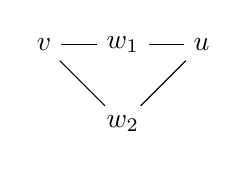
\begin{tikzpicture}
				\graph { v/$v$ -- {w1/$w_1$, w2/$w_2$} -- u/$u$ };
			\end{tikzpicture}
			\she
		\end{center}
		
		נבחין ש־: 
		\[ v \to w_1 \to u \to w_2 \to v \to w_1 \to u \]
		הוא מסלול $v \squig u$ באורך $7$ על אף שישנו מסלול קצר יותר בינהם, דהיינו הוא איננו מק''ב. זאת על אף שהגרף לעיל הוא גרף המק''בים $G^*_{u, v}$ של עצמו, כי עליו לכלול את המסלולים $v \to w_1 \to u$ ו־$v \to w_2 \to u$ שהם המק''בים מ־$v$ ל־$u$. סתירה. 
	\end{enumerate}
	
	\npage
	\section{}
	בהינתן חלוקת קשתות של $G = (V, E)$ לאדום ולכחול, ו־$s, t$: 
	\begin{enumerate}[A.]
		\item נמצא מסלול מינימלי $s \squig t$ שעובר דרך מספר מינימלי של קשתות אדומות. [\textit{הערה לבודק:} חשבתי ''למשקל`` תוך ריצת ה־BFS מעבר בקשתות אדומות כמרחק של $\sof V$, אבל הפתרון הזה לא ממש עובד עם הסעיף הבא]
		\begin{itemize}
			\item \textbf{אלגוריתם: }נגדיר את $G|_B$ (''הצמצום לגרף כחול``) להיות הגרף $G|_B = (V, E|_B)$ כאשר $E|_B$ כולל רק את הקשתות הכחולות. נמצא את רכיבי הקשירות בו (לדוגמה באמצעות BFS) ונסמנם $C_1 \dots C_n$ (בה''כ $s \in C_1, t \in C_n$). נגדיר ''גרף על`` שנסמנו $G|_B^*$ להיות הגרף שצמתיו הם רכיבי הקשירות $c_1 \dots C_n$, וקשתותיו הן הקשתות $\{v, u\}$ האדומות שמחברות $v \in C_i$ כלשהו ל־$u \in C_{j}$ כלשהו. נריץ BFS בגרף זה בין $C_1$ ל־$C_n$, למציאת מסלול קצר ביותר של קשתות אדומות, ואז בעבור כל $C_i$ שמופיע במסלול, נריץ BFS למציאת המסלול הקצר ביותר של קשתות כחולות בין הצומת ממנה נכנסו ל־$C_i$ לבין הצומת ממנה יצאנו. לבסוף נחזיר את שרשור המסלולים. 
			
			\item \textbf{סיבוכיות: }אומנם אנחנו מריצים BFS על מספר לא ידוע של רכיבי קשירות, אבל סך הקשתות שנסרקות ע''י ה־BFS־ים הכחולים הוא $\sof{E|_B}$ וסך הצמתים הוא $\sof V$, וסך הקשתות הנסרקות ע''י ה־BFS האדום הוא $\sof{E|_R}$ (הצמצום לקשתות אדומות) וסך הצמתים $\sof V$. סה''כ $\oc(\sof{E|_B} + \sof{E|_R} + 2\sof V) = \oc(\sof E + \sof V)$. 
			
			\item \textbf{נכונות: }בבירור מוחזר מסלול $s \squig t$, נוכיח שיש בו מספר מינימלי של קשתות כחולות. נתבונן במסלול מינימלי כלשהו של קשתות אדומות. כל רצף של קשתות כחולות במסלול ישתייך לאותו רכיב קשירות שנסמן ב־$C_i$, כי אם הם יהיו מפורדים במסלול: 
			\[ v_1 \to u_1 \squig u_2 \to v_2 \squig v_3 \to u_3 \squig u_4 \to v_4 \]
			כאשר $u_1 \squig u_2, u_3 \squig u_4$ תתי מסלולים כחולים ששייכים לאותו רכיב הקשירות, ו־$v_2 \squig v_3$ מסלול אדום, נוכל להחליף את $v_2 \squig v_3$ במסלול $u_1 \squig u_4$ במקום, וליצור מסלול עם פחות צמתים אדומים מזה שהתחלנו ממנו, בסתירה להנחה שהוא מינימלי (ביחס למספר צמתים אדומים). מכאן שאותו המסלול המינימלי יכול לבוא לידי ביטוי בגרף העל $G|_B^*$ כמסלול אדום בין רכיבי קשירות, ולכן הוא באותו האורך כמו המסלול שה־BFS מצא. 
		\end{itemize}
		
		\item מבין כל המסלולים עם מספר מינימלי של קשתות אדומות, נמצא את זה עם מספר מינימלי של קשתות כחולות. 
		\begin{itemize}
			\item \textbf{אלגוריתם: }נבצע את אותה הבנייה כמו בסעיף הקודם, אך נמצא את גרף המק''בים בין $C_1$ ל־$C_n$ בגרף העל $G|_B^*$ במקום למצוא מסלול בודד. לאחר מכן נמצא גרף מק''בים בעבור כל רכיב קשירות $C_i$. נחזור ל־$G$ ונשאיר בו את הקשתות שנמצאות בגרפי המ''קבים השונים, ליצירת גרף $G'$. נריץ BFS ב־$G'$ ונחזיר את התוצאה. 
			
			\item \textbf{סיבוכיות: }שקול לניתוח הסיבוכיות של הסעיף הקודם, שכן מציאת גרף מק''בים בגרף לא מכוון פועלת בדומה ל־BFS. 
			\item \textbf{נכונות: }
			\begin{itemize}
				\item ראשית נראה שהמסלול הוא מינימלי במספר הקשתות האדומות. בין כל המק''בים בין $s$ ל־$t$ ב־$G'$ מופיע אותה כמות (מינימלית) של קשתות אדומות. זאת כי אם המק''ב לא חוזר על אותו רכיב הקשירות פעמיים, אז זה שקול ללהסתכל עליו קשתותיו האדומות כעל מק''ב בגרף העל $G|_B^*$, ואם הוא כן, זו סתירה באמצעות נימוק זהה לנימוק שהפעלנו בסעיף קודם. 
				\item שנית נראה נראה שבמסלול מספר קשתות כחולות מינימלי (מבין המק''בים עם מספר קשתות אדומות מינימלי). מהגדרת גרף המק''בים ובגלל שהראנו שמספר הקשתות האדומות בכל מק''ב ב־$G'$ קבוע, בהכרח כל מק''ב ב־$G'$ יהיה מק''ב עםמספר קשתות אדומות מינימלי, וכל מק''ב עם מספר קשתות אדומות מינימלי יהיה ב־$G'$. מכאן שמסלול קצר ביותר עם מספר קצר ביותר בגרף זה היה מסלול עם מספר קשתות כחולות מינימלי (מבין המק''בים הרלוונטיים) כנדרש. 
			\end{itemize}
		\end{itemize}
		
		\textit{הערה לבודק: }– לא ברור לי איך הרמז מועיל. 
	\end{enumerate}
	
	
	\ndoc
\end{document}
